\documentclass{article}
%%%%%%%%%%%%%%%%%%%%%%%%%%%%% Define Article %%%%%%%%%%%%%%%%%%%%%%%%%%%%%%%%%%
%%%%%%%%%%%%%%%%%%%%%%%%%%%%%%%%%%%%%%%%%%%%%%%%%%%%%%%%%%%%%%%%%%%%%%%%%%%%%%%

%%%%%%%%%%%%%%%%%%%%%%%%%%%%% Using Packages %%%%%%%%%%%%%%%%%%%%%%%%%%%%%%%%%%
\usepackage{float}
\usepackage[letterpaper,portrait]{geometry}
\usepackage{graphicx}
\usepackage{anysize}
\usepackage{lipsum}
\usepackage{amsmath,amssymb,amsthm}
\usepackage[utf8]{inputenc}
\usepackage{multirow}
\usepackage{csquotes}
\usepackage[spanish]{babel}
\usepackage{apacite}
\usepackage{multicol}
\usepackage{parskip}
\usepackage{setspace}
\usepackage{empheq}
\usepackage{mdframed}
\usepackage{booktabs}
\usepackage{lipsum}
\usepackage{graphicx}
\usepackage{color}
\usepackage{psfrag}
\usepackage{pgfplots}
\usepackage{bm}
\usepackage{tocloft}
\usepackage{lscape}
\usepackage{adjustbox}
%%%%%%%%%%%%%%%%%%%%%%%%%%%%%%%%%%%%%%%%%%%%%%%%%%%%%%%%%%%%%%%%%%%%%%%%%%%%%%%

% Other Settings

%%%%%%%%%%%%%%%%%%%%%%%%%% Page Setting %%%%%%%%%%%%%%%%%%%%%%%%%%%%%%%%%%%%%%%
\geometry{letterpaper, margin=2.54cm}

%%%%%%%%%%%%%%%%%%%%%%%%%% Define some useful colors %%%%%%%%%%%%%%%%%%%%%%%%%%
\definecolor{ocre}{RGB}{243,102,25}
\definecolor{mygray}{RGB}{243,243,244}
\definecolor{deepGreen}{RGB}{26,111,0}
\definecolor{shallowGreen}{RGB}{235,255,255}
\definecolor{deepBlue}{RGB}{61,124,222}
\definecolor{shallowBlue}{RGB}{235,249,255}
%%%%%%%%%%%%%%%%%%%%%%%%%%%%%%%%%%%%%%%%%%%%%%%%%%%%%%%%%%%%%%%%%%%%%%%%%%%%%%%

%%%%%%%%%%%%%%%%%%%%%%%%%% Define an orangebox command %%%%%%%%%%%%%%%%%%%%%%%%
\newcommand\orangebox[1]{\fcolorbox{ocre}{mygray}{\hspace{1em}#1\hspace{1em}}}
%%%%%%%%%%%%%%%%%%%%%%%%%%%%%%%%%%%%%%%%%%%%%%%%%%%%%%%%%%%%%%%%%%%%%%%%%%%%%%%

%%%%%%%%%%%%%%%%%%%%%%%%%%%% English Environments %%%%%%%%%%%%%%%%%%%%%%%%%%%%%
\newtheoremstyle{mytheoremstyle}{3pt}{3pt}{\normalfont}{0cm}{\rmfamily\bfseries}{}{1em}{{\color{black}\thmname{#1}~\thmnumber{#2}}\thmnote{\,--\,#3}}
\newtheoremstyle{myproblemstyle}{3pt}{3pt}{\normalfont}{0cm}{\rmfamily\bfseries}{}{1em}{{\color{black}\thmname{#1}~\thmnumber{#2}}\thmnote{\,--\,#3}}
\theoremstyle{mytheoremstyle}
\newmdtheoremenv[linewidth=1pt,backgroundcolor=shallowGreen,linecolor=deepGreen,leftmargin=0pt,innerleftmargin=20pt,innerrightmargin=20pt,]{theorem}{Theorem}[section]
\theoremstyle{mytheoremstyle}
\newmdtheoremenv[linewidth=1pt,backgroundcolor=shallowBlue,linecolor=deepBlue,leftmargin=0pt,innerleftmargin=20pt,innerrightmargin=20pt,]{definition}{Definition}[section]
\theoremstyle{myproblemstyle}
\newmdtheoremenv[linecolor=black,leftmargin=0pt,innerleftmargin=10pt,innerrightmargin=10pt,]{problem}{Problem}[section]
%%%%%%%%%%%%%%%%%%%%%%%%%%%%%%%%%%%%%%%%%%%%%%%%%%%%%%%%%%%%%%%%%%%%%%%%%%%%%%%

%%%%%%%%%%%%%%%%%%%%%%%%%%%%%%% Plotting Settings %%%%%%%%%%%%%%%%%%%%%%%%%%%%%
\usepgfplotslibrary{colorbrewer}
\pgfplotsset{width=8cm,compat=1.9}
%%%%%%%%%%%%%%%%%%%%%%%%%%%%%%%%%%%%%%%%%%%%%%%%%%%%%%%%%%%%%%%%%%%%%%%%%%%%%%%

%%%%%%%%%%%%%%%%%%%%%%%%%%%%%%% Title & Author %%%%%%%%%%%%%%%%%%%%%%%%%%%%%%%%
\author{Gustavo Vergara}
%%%%%%%%%%%%%%%%%%%%%%%%%%%%%%%%%%%%%%%%%%%%%%%%%%%%%%%%%%%%%%%%%%%%%%%%%%%%%%%

\begin{document}
\pgfplotsset{compat=1.18}
\setstretch{2}

\begin{titlepage}
	\centering
	\vspace{2.5cm}
	{\scshape \Large Elaboración de los diagramas del modelo de dominio del proyecto - GA2-220501093-AA2-EV01 \par}
	\vspace{5cm}
	\textbf\large\scshape{\par}
	\vspace{0.5cm}

	{\Large Vergara Pareja Gustavo\par}
	\vspace{5cm}
	{\scshape\Large Jovanna Herazo\par}
	\vspace{0.3cm}
	{\scshape\Large Tecnología en Análisis y Desarrollo de Software \par}
	\vspace{0.3cm}
	{\scshape\Large SENA - Centro Agropecuario Regional Cauca\par}
	\vspace{0.3cm}
	{\Large \today \par}
\end{titlepage}
\tableofcontents
\newpage

\large \textbf{ACTIVIDAD A SOLUCIONAR}\\
\vspace{0.1cm}
\section*{TALLER INSTRUMENTOS - METROLOGÍA Y CONTROL DE CALIDAD}
\section{¿Qué es el calibrador Vernier o pie de rey?}
Es un instrumento de medida de uso muy común por su fácil manejo y el grado de precisión en las mediciones realizadas. Básicamente, consta de una regla (graduada en milímetros) con una escuadra o tacón en el origen que determina la boca fija, sobre la que se desplaza
una pequeña regla móvil (nonio) que en su origen determina la boca móvil. El calibrador típico puede tomar tres tipos de mediciones: exteriores,
interiores y profundidades, pero algunos además pueden realizar medición de peldaño.
\begin{enumerate}
\item ¿Cuántos modelos de vernier existen?\newline
Los vernier se clasifican en tres tipos, el estándar, largo y en pulgadas.
\begin{itemize}
\item Vernier estándar \newline
Este tipo de vernier es el más comúnmente utilizado, tiene n divisiones iguales
que ocupan la misma longitud que n-1 divisiones sobre la escala principal.
\begin{figure}[H]
	\centering
	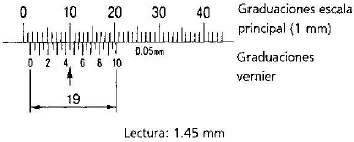
\includegraphics[width=0.6\textwidth]{lectura_vernier.png}
	\caption{Vernier estándar}
	\label{fig:imagen2}
\end{figure}
\end{itemize}

\begin{itemize}
	\item Vernier largo \newline
	      El vernier largo está diseñado para que las graduaciones adyacentes sean más
	      fáciles de distinguir.
	      \begin{figure}[H]
		      \centering
		      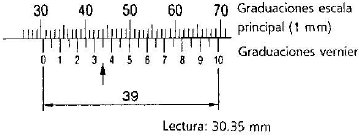
\includegraphics[width=0.6\textwidth]{lectura2.png}
		      \caption{Vernier Largo}
		      \label{fig:imagen2}
	      \end{figure}
		\end{itemize}

		\begin{itemize}
			\item Vernier en pulgadas 
			\newline
				  El vernier en pulgadas utiliza la misma metododología del vernier estandar.
				  \begin{figure}[H]
					  \centering
					  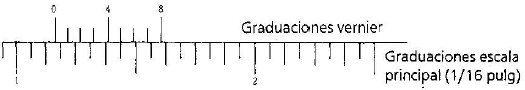
\includegraphics[width=0.6\textwidth]{vpulg.png}
					  \caption{Vernier en pulgadas}
					  \label{fig:imagen2}
				  \end{figure}
				\end{itemize}

\item ¿Para qué sirve cada uno?\newline
Si nos referimos a modelos, hay dos: analógico y digital
\begin{itemize}
	\item Vernier analogico \newline
	Este tipo de calibrador tiene una escala vernier que debe leerse manualmente.
	\begin{figure}[H]
		\centering
		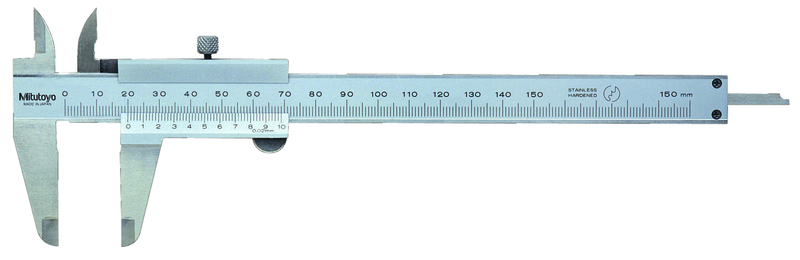
\includegraphics[width=0.6\textwidth]{ss.png}
		\caption{Vernier analógico}
		\label{fig:imagen2}
	\end{figure}
\end{itemize}
\begin{itemize}
	\item Vernier digital \newline
	Este tipo de calibrador tiene una pantalla digital que muestra la medida directamente.
	\begin{figure}[H]
		\centering
		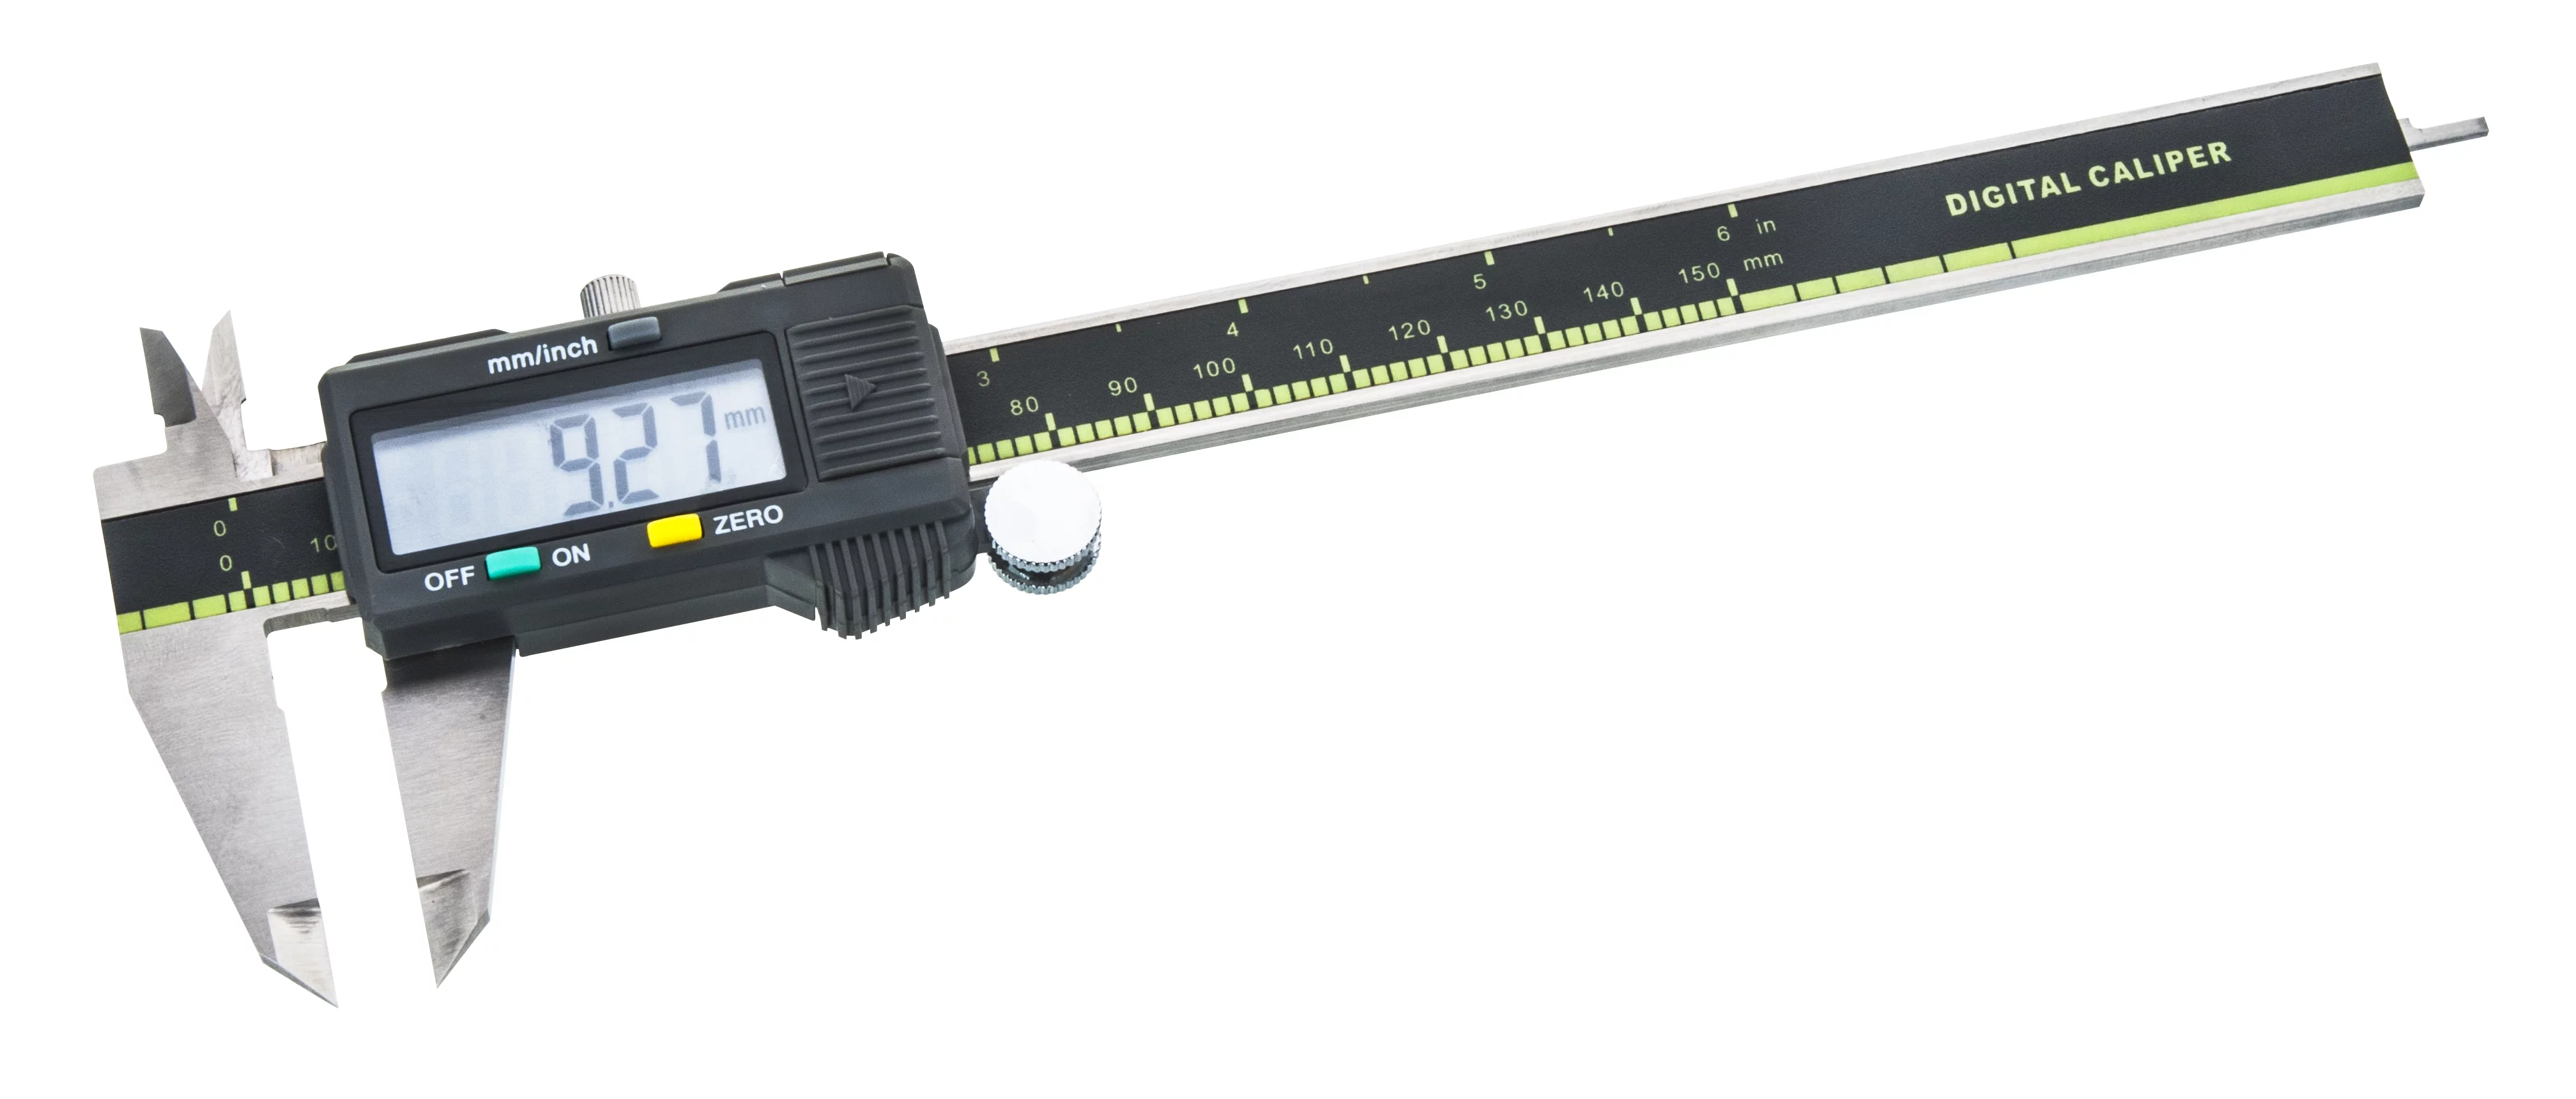
\includegraphics[width=0.6\textwidth]{digi.png}
		\caption{Vernier digital}
		\label{fig:imagen2}
	\end{figure}
\end{itemize}
\item ¿Cuáles son sus partes?

\item ¿Cómo se lee la medida en el instrumento?
\end{enumerate}
\section{¿Qué es el micrómetro?}
\begin{itemize}
	\item ¿Cuáles son sus partes?

	\item¿Cómo se lee la medida en el instrumento?

	\item¿Qué es el micrómetro?

	\item¿Cuántos modelos de micrómetros existen?

	\item¿Para qué sirve cada uno?

	\item¿Cuáles son sus partes?
\end{itemize}

\newpage

\begin{figure}[H]
	\centering
	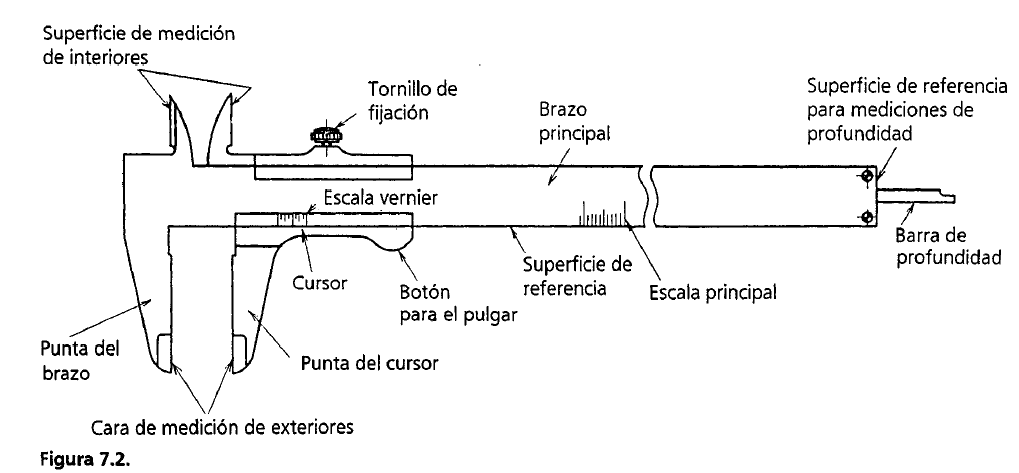
\includegraphics[width=1\textwidth]{partes_vernier.png}
	\caption{Diagrama de paquetes}
	\label{fig:imagen2}
\end{figure}
Es un instrumento de medición que se utiliza para medir longitudes, diámetros, profundidades
y espesores con una precisión de hasta 0,02 mm. Fué elaborado para satisfacer la necesidad
de un instru­mento de lectura directa que pudiera brindar una medida fácilmente, en una sola
operación. El calibrador típico puede tomar tres tipos de mediciones: exteriores,
interiores y profundidades, pero algunos además pueden realizar medición de peldaño.

\end{document}